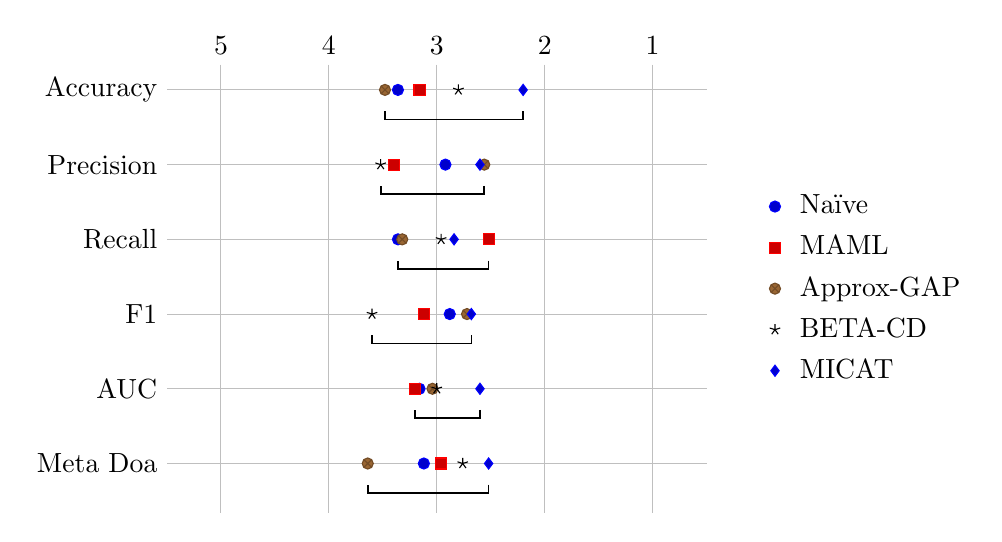
\begin{tikzpicture}[
  group line/.style={semithick},
]

\begin{axis}[
  clip={false},
  grid={both},
  axis line style={draw=none},
  tick style={draw=none},
  xticklabel pos={upper},
  y dir={reverse},
  xmin={0.5},
  ymin={0.66},
  legend style={draw=none,fill=none,at={(1.1,.5)},anchor=west,row sep=.25em,/tikz/every odd column/.append style={column sep=.5em}},
  legend cell align={left},
  title style={yshift=\baselineskip},
  width={\axisdefaultwidth},
  ytick={1,2,3,4,5,6},
  yticklabels={{Accuracy},{Precision},{Recall},{F1},{AUC},{Meta Doa}},
  xmax={5.5},
  ymax={6.66},
  height={1.0*\axisdefaultheight},
  x dir={reverse},
  title={},
]

\addplot+[only marks] coordinates {
  (3.36, 1)
  (2.92, 2)
  (3.36, 3)
  (2.88, 4)
  (3.16, 5)
  (3.12, 6)
};
\addlegendentry{Naïve}
\addplot+[only marks] coordinates {
  (3.16, 1)
  (3.4, 2)
  (2.52, 3)
  (3.12, 4)
  (3.2, 5)
  (2.96, 6)
};
\addlegendentry{MAML}
\addplot+[only marks] coordinates {
  (3.48, 1)
  (2.56, 2)
  (3.32, 3)
  (2.72, 4)
  (3.04, 5)
  (3.64, 6)
};
\addlegendentry{Approx-GAP}
\addplot+[only marks] coordinates {
  (2.8, 1)
  (3.52, 2)
  (2.96, 3)
  (3.6, 4)
  (3.0, 5)
  (2.76, 6)
};
\addlegendentry{BETA-CD}
\addplot+[only marks] coordinates {
  (2.2, 1)
  (2.6, 2)
  (2.84, 3)
  (2.68, 4)
  (2.6, 5)
  (2.52, 6)
};
\addlegendentry{MICAT}
\draw[group line] (axis cs:2.2,1.2832618025751072) -- ++(0pt,-3pt) -- ([yshift=-3pt]axis cs:3.48,1.2832618025751072) -- ++(0pt,3pt);
\draw[group line] (axis cs:2.56,2.2832618025751072) -- ++(0pt,-3pt) -- ([yshift=-3pt]axis cs:3.52,2.2832618025751072) -- ++(0pt,3pt);
\draw[group line] (axis cs:2.52,3.2832618025751072) -- ++(0pt,-3pt) -- ([yshift=-3pt]axis cs:3.36,3.2832618025751072) -- ++(0pt,3pt);
\draw[group line] (axis cs:2.68,4.283261802575107) -- ++(0pt,-3pt) -- ([yshift=-3pt]axis cs:3.6,4.283261802575107) -- ++(0pt,3pt);
\draw[group line] (axis cs:2.6,5.283261802575107) -- ++(0pt,-3pt) -- ([yshift=-3pt]axis cs:3.2,5.283261802575107) -- ++(0pt,3pt);
\draw[group line] (axis cs:2.52,6.283261802575107) -- ++(0pt,-3pt) -- ([yshift=-3pt]axis cs:3.64,6.283261802575107) -- ++(0pt,3pt);

\end{axis}
\end{tikzpicture}